\documentclass[10pt,doublecolumn]{IEEEtran}  % Comment this line out if you need a4paper
%\documentclass[a4paper, 10pt, conference]{ieeeconf}      % Use this line for a4 paper

\usepackage{epsfig}
\usepackage{epstopdf}
\usepackage[cmex10]{amsmath}
\usepackage{amssymb}
\usepackage{array}
\usepackage{mdwmath}
\usepackage{mdwtab}
\usepackage{cases}
\usepackage{eqparbox}
\usepackage{subfig}
\usepackage{color}

\IEEEoverridecommandlockouts
% This command is only needed if% you want to use the \thanks command
\overrideIEEEmargins                                      
% Needed to meet printer requirements.

% See the \addtolength command later in the file to balance the column lengths
% on the last page of the document

% The following packages can be found on http:\\www.ctan.org
%\usepackage{graphics} % for pdf, bitmapped graphics files
%\usepackage{epsfig} % for postscript graphics files
%\usepackage{mathptmx} % assumes new font selection scheme installed
%\usepackage{times} % assumes new font selection scheme installed
%\usepackage{amsmath} % assumes amsmath package installed
%\usepackage{amssymb}  % assumes amsmath package installed

%\title{\LARGE \bf
%Distributed $\varepsilon$-Nash Strategies for Multi-Agent Formation Control}
%
%
%\author{Wei~Lin$^\dag$,~\IEEEmembership{Student Member,~IEEE,}
%        Zhihua~Qu$^\dag$,~\IEEEmembership{Fellow,~IEEE,}
%        and~Marwan~A. Simaan$^\dag$,~\IEEEmembership{Life Fellow,~IEEE}
%% <-this % stops a space
%\thanks{*This work is supported in part by US National Science Foundation under grants ECCS-1308928 and CCF-0956501 as well as by US Department of Energy's award DE-EE0006340 under the Grid Engineering for Accelerated Renewable Energy Deployment (GEARED) program and another subcontract under the Solar Energy Grid Integration Systems (SEGIS) program (phases I to III).}% <-this % stops a space
%\thanks{$^\dag$Wei Lin, Zhihua Qu, and Marwan A. Simaan are with the Department of EECS, University of Central Florida, Orlando, Florida, 32816, USA. Emails:
%        {\tt\small weilin0929@gmail.com, qu@eecs.ucf.edu, simaan@eecs.ucf.edu}.}%
%%
%}

\begin{document}
\title{\LARGE \bf
Distributed Game Strategy Design with Application to Multi-Agent Formation Control}


\author{Wei~Lin,~\IEEEmembership{Member,~IEEE,}
        Zhihua~Qu~\IEEEmembership{Fellow,~IEEE,},~and
        Marwan~A. Simaan,~\IEEEmembership{Life Fellow,~IEEE}
% <-this % stops a space
\thanks{This work is supported in part by US National Science Foundation under grants ECCS-1308928 and CCF-0956501, by US Department of Energy’s award DE-EE0006340, by US Department of Transportation’s award DTRT13-G-UTC51, by L-3 Communication’s contract 11013I2034, and by Leidos’ contract P010161530.}% <-this % stops a space
\thanks{Wei Lin is with Western Digital Corporation, Irvine, CA, 92612, USA. E-mail: weilin0929@gmail.com.}
\thanks{Zhihua Qu and Marwan A. Simaan are with the Department of EECS, University of Central Florida, Orlando, Florida, 32816, USA, e-mails: qu@eecs.ucf.edu, simaan@eecs.ucf.edu.}%
%
}


%\markboth{Journal of \LaTeX\ Class Files,~Vol.~11, No.~4, December~2012}%
%{Shell \MakeLowercase{\textit{et al.}}: Bare Demo of IEEEtran.cls for Journals}

\maketitle

\IEEEpeerreviewmaketitle

%%%%%%%%%%%%%%%%%%%%%%%%%%%%%%%%%%%%%%%%%%%%%%%%%%%%%%%%%%%%%%%%%%%%%%%%%%%%%%%%
\begin{abstract}
In this paper, we consider a multi-agent formation control problem from a game theory point of view. It is well known that a major difficulty in a communication network based formation control problem is that each agent is only able to exchange information with other agents according to the communication topology. This information constraint prevents many game strategy design approaches that require individual agents to have global information from being implemented in many cases. We formulate the formation control problem in such a way that individual agents try to minimize their locally measured formation errors and to solve it as a differential game problem. We consider two cases of non-cooperative and cooperative games and propose a novel distributed design approach that utilizes the relationship between the initial and terminal state variables. This approach is applied to an illustrative formation control example among three agents and the formation errors under various scenarios are compared and analyzed.
\end{abstract}

\newtheorem{Def}{Definition}
\newtheorem{Asu}{Assumption}
\newtheorem{thm}{Theorem}
\newtheorem{Pro}{Proposition}
\newtheorem{Alg}{Algorithm}
\newtheorem{Lem}{Lemma}
\newtheorem{Rmk}{Remark}
\newtheorem{Cor}{Corollary}

\section{Introduction}
An important application of cooperative control theory \cite{ren,Qu} is the multi-agent formation control problems \cite{Stipanovic2004,Keviczky2008,JiananWang2012}. This problem revolves around designing  local information constrained control inputs for the agents (mobile robots, unmanned vehicles, etc) and making their positions follow a prescribed formation. There  is considerable work  done in this field and the comprehensive review paper \cite{Cao2013} on multi-agent distributed control systems is a good reference on recent progress in cooperative control theory including the formation control problem. Recently, multiple attempts \cite{anderson1998formation,DongbingGu2008,SemsarKazerooni20092205} have been made to incorporate differential  game theory \cite{Isaacs,Basar} into the formation control design problem. A fundamental connection between these two problems can be explained as follows: in a multi-agent formation control problem, all the agents are basically trying to minimize the formation errors between each other. If every agent is able to observe all the other agents, then the problem can be essentially viewed as an optimal control problem where a common performance index of global formation errors can be assigned for all the agents. However, in most of realistic applications, since the agents are usually connected through a communication network  with  a certain topology, they are only able to exchange information with each other in a distributed manner (i.e., to share information locally). In this case, instead of minimizing a globally defined performance index, it is  more realistic  for each agent to only minimize a performance index of its locally measured formation errors. This scenario is exactly equivalent to that of a differential game where each player is trying to minimize its own performance index. Therefore, most  multi-agent  formation control design  problems  can be viewed and solved as  differential game problems . The game solutions including  Nash equilibria for non-cooperative agents and Pareto optimality for cooperative agents can be well established. However, solving  for  the Nash and Pareto solutions under distributed information is not a trivial task in the multi-agent environment because of the following two  issues : (1) the strategy for each agent has to conform to its local information topology constraint and (2) local strategy computing within each agent is preferred rather than centralized strategy computing where strategies are designed by a centralized designer and assigned to individual agents.  In \cite{DongbingGu2008,SemsarKazerooni20092205}, the first  issue  has been addressed and the corresponding Nash and Pareto strategies are considered for the formation control problem as a differential game. In this present paper, we will focus more on the second aspect. By investigating the structure of the game solution in more details, a strategy design approach as well as an implementation algorithm are proposed for each agent to carry out its optimal control strategy design in a fully distributed manner. The remainder of this paper is organized as follows. A brief setup of the game problem is presented in Section \ref{setup}. The main results of the distributed Nash and Pareto strategy designs are presented in Section \ref{mainresult1} and \ref{mainresult2} respectively. An illustrative example with three agents under noncooperative and cooperative cases is presented and analyzed in Section \ref{simulation}.


%%%%%%%%%%%%%%%%%%%%%%%%%%%%%%%%%%%%%%%%%%%%%%%%%%%%%%%%%%%%%%%%%%%%%%%%%%%%%%%%
\section{Problem Formulation}\label{setup}
We consider the finite-time formation control problem between $N$ agents in the $n$-dimensional Euclidean space where the motion dynamics of each agent is described as the following double integrator model:
\begin{equation}
\begin{bmatrix}
\dot{p}_i\\ \dot{v}_i
\end{bmatrix}=\begin{bmatrix}
0&I_n\\0&0
\end{bmatrix}\begin{bmatrix}
p_i\\
v_i\end{bmatrix}+\begin{bmatrix}
0\\ I_n
\end{bmatrix}u_i\label{systemxi}
\end{equation}
for $i=1,\cdots,N$. Vector $p_i\in\mathbb{R}^n$ and $v_i\in\mathbb{R}^n$ are the position and velocity of agent $i$ respectively. Vector $u_i\in\mathbb{R}^{n}$ is the acceleration control of agent $i$. We assume that the agents are able to exchange information with each other through a communication network {whose topology can be described by a set $\mathcal{E}$ in graph theory. An edge $e_{ij}\in\mathcal{E}$ represents information being transmitted from agent $j$ to agent $i$}. The objective of the agents is to form a prescribed formation over a finite time interval, which is equivalent to individual agents minimizing the following performance indices:

Since every agent is only aware of its local communication pattern and its own performance index, this formation problem can be regarded as a differential game problem where each player {has} its own objectives to pursue over a time interval. In this paper, we consider two types of open-loop {(where the control inputs are functions of initial states and time only)} formation control approaches through {differential} game strategy design. Specifically, {if the control inputs $u_1,\cdots,u_N$ can be looked as strategies}, then for the formulated problem, strategies {$u^{N}_{1},\cdots,u^{N}_N$} are the Nash strategies and form a Nash equilibrium if the inequality
\begin{align}
&{J_{i}(u_1^{N},\cdots,u^{N}_i,\cdots,u^{N}_N)\leq J_{i}(u_1^{N},\cdots,u_i,\cdots,u^{N}_N)}\label{Nashinequality}
\end{align}
holds for all $u_i\in U_i$ and for all $i=1,\cdots,N$, where $U_i$ is the open-loop control set for agent $i$, i.e., $U_i=\{u_i(t,x(0))\in \mathbf{R}^r \mid t\in[0,t_f]\}$. The Nash equilibrium is an equilibrium where it is not possible for any agent to lower its performance index value by unilaterally deviating from its Nash strategy. The Nash equilibrium is a widely used solution in the situation where the players do not {cooperate} with each other. On the other hand, The strategies $u^{P}_0,u^{P}_{1},\cdots,u^{P}_N$ are the Pareto strategies and {form a Pareto optimality if the inequality
\begin{align}
&J_{i}(u^P_1,\cdots,u^P_N)< J_{i}(u_1,\cdots,u_N) \label{inequality}
\end{align}
holds for at least one $i\in\{1,\cdots,N\}$.} The Pareto optimality can be interpreted as a solution in which any changes made do not help lower every agent's performance index value. The Pareto optimality is a widely used solution in the situation where the players can {cooperate} with each other. In the following sections, two formation control approaches will be proposed based on the open-loop Nash strategy (assuming that the agents do not {cooperate}) and the open-loop Pareto strategy (assuming that the agents {cooperate}).
%%%%%%%%%%%%%%%%%%%%%%%%%%%%%%%%%%%%%%%%%%%%%
\section{Open-Loop Nash Analysis for Homogeneous Agents}
We consider homogeneous time varying discrete time agents' dynamics:
\begin{align*}
&\dot{x}_i(t)=A_i(t)x_i(t)+B_i(t)u_i(t)\\
&y_{i}(t)=C_i(t)x_i(t)
\end{align*}
where $y_i\in\mathbf{R}^m$ is the output state of agent $i$ that needs to be coordinated with other agents, such as velocity, position, etc. The initial state $x_i(0)$ is usually known to agent $i$ only. To further simplify the problem, we define a new state vector as
\begin{equation}
z_i=C_i(t)\Phi_i(t_f,t)x_i(t)\label{zi}
\end{equation}
where $\Phi_i(t_f,t)=e^{A_i(t_f-t)}$ is the state-transition matrix. Differentiating the above equation with
respect to $t$ yields:
\begin{align}
\dot{z}_i=&C_i\dot{\phi}_ix_i+C_i\phi_i\dot{x}_i \notag\\
=&B_iu_i ,\label{zidot}
\end{align}
where $B'_i=C_i\phi_i(t_f,t)B_i$.

The objective of a coordination problem among multiple agents is generally equivalent to minimizing by the following performance index
\begin{align}
J_i=&\frac{1}{2}\sum_{e_{ij}\in\mathcal{E}} [y_i(t_f)-y_j(t_f)-\mu_{ij}]^TF_{ij}[y_i(t_f)-y_j(t_f)-\mu_{ij}]\notag \\
&+\frac{1}{2}\int_{0}^{t_f} u_i^TR_iu_idt \label{JiFormation}
\end{align}
for $i=1,\cdots,N$, where $\mu_{ij}$ is a prescribed vector by the coordination problem, matrix $F_{ij}$ is positive-semi definite, and matrix $R_i(t)$ is positive definite for all $t\in[0,t_f]$. Minimizing performance index $J_i$ means that every agent will try to minimize its total coordination error measured locally according to the graph while at the same time minimizing its total control energy in the game. To facilitate Nash strategy analysis for the formulated multi-agent coordination problem, we define a matrix weighted Laplacian based on network topology and agents' performance indices.
\begin{Def}
For the multi-agent coordination problem on graph $\mathcal{G}$ with performance indices in (\ref{JiFormation}), a \textbf{matrix weighted Laplacian matrix} is defined as $L=[L_{ij}]\in\mathbb{R}^{Nn\times Nn}$ where
\begin{equation}
L_{ij}=\left\{\begin{array}{ll}
-C^TF_{ij}C&\mbox{if $e_{ij}\in\mathcal{E}$ and $j\neq i$}\\
0&\mbox{if $e_{ij}\notin\mathcal{E}$ and $j\neq i$}\\
\displaystyle \sum_{e_{ij}\in\mathcal{E}}C^TF_{ij}C&\mbox{if $j=i$}
\end{array}\right..\label{laplacian}
\end{equation}
\end{Def}




The open-loop Nash equilibrium for the formulated problem is presented as follows.
\begin{thm}
For the $N$-agent linear quadratic differential game of fixed duration $[0,t_f]$ defined by agents' dynamics (\ref{systemxi}) and performance indices (\ref{JiFormation}), if the information structure of every agent is open-loop, i.e., $U_i=\{u_i(t,x(0))\in \mathbf{R}^r \mid t\in[0,t_f]\}$, there exists a unique Nash equilibrium where corresponding open-loop control strategy vector $u^*_i$ is given by
\begin{align}
&u_i^*=-R_i^{-1}B^T [e_i\otimes\Phi^T(t_f,t)] \{L(I+DL)^{-1}\notag\\
&[\Phi(t_f,0)x(0)+D\mu]-\mu\}\label{uNash}
\end{align}
if matrix $(I+DL)$ is invertible, where $e_i$ is a vector with the $i$th entry being 1 and elsewhere 0
\begin{align}
D=&\begin{bmatrix}
D_1&&\\
&\ddots&\\
&&D_N
\end{bmatrix},
x=\begin{bmatrix}
x_1\\
\vdots\\
 x_N
\end{bmatrix},
\mu=\begin{bmatrix}
\sum_{e_{1j}\in{\mathcal{E}}}\mu^T_{1j}\\
\vdots\\
\sum_{e_{Nj}\in{\mathcal{E}}}\mu^T_{Nj}
\end{bmatrix},\notag\\
D_i=&\int^{t_f}_0\Phi(t_f,\tau)B_iR_i^{-1}B_i^T\Phi^T(t_f,\tau) dt
.\label{Di} 
\end{align}
\end{thm}

\begin{proof}
We define the Hamiltonian for agent $i$ as
\begin{align}
H_i=&\frac{1}{2}u_i^TR_iu_i+ \lambda_{i}^T(A_ix_i+B_iu_i)
\end{align}
where vector $\lambda_i$ is the Lagrangian multiplier. Necessary conditions for the existence of open-loop Nash equilibria are
\begin{subequations}\begin{align}
\dot{x}_{i}=&\frac{\partial H_i}{\partial \lambda_{i}}=A_ix_i+B_iu_i,\label{Nec1}\\ 
\dot{\lambda}_{i}=&-\frac{\partial H_i}{\partial x_{i}}= -A_i^T\lambda_i,\label{Nec2}\\
\lambda_{i}(t_f)=& \sum_{e_{ij}\in\mathcal{E}} C_i^TF_{ij}C_i[x_i(t_f)-x_j(t_f)-\mu_{ij}]\notag\\
=& \sum_{e_{ij}\in\mathcal{E}} L_{ij}[x_i(t_f)-x_j(t_f)]-\mu_i,\label{Nec3}\\
\frac{\partial H_i}{\partial u_i}=&R_iu_i+B^T_i\lambda_i =0,\label{Nec4}
\end{align}\label{Nec}
\end{subequations}
for all $i=1,\cdots,N$, where $\mu_i=\sum_{e_{ij}\in\mathcal{E}}C^TF_{ij}\mu_{ij}$. Therefore, the existence of the Nash equilibria is equivalent to the solvability of above equations given initial states $x_i(0)$ for all $i=1,\cdots,N$. The uniqueness of Nash equilibrium is equivalent to the uniqueness of the solution to conditions (\ref{Nec1}) to (\ref{Nec4}). From (\ref{Nec2}), the trajectory of $\lambda_i$ can be obtained as
\[\lambda_i(t)=\Phi_i^T(t_f,t)\lambda_i(t_f)\]
where $\Phi(t_f,t) = e^{A(t_f-t)}$. From (\ref{Nec4}), the control vector can be obtained as
\begin{align}
u_i(t)=-R_i^{-1}B^T\lambda_i(t),\label{ulambda}
\end{align}
Substituting the above expression into (\ref{Nec1}) yields
\[\dot{x}_i=Ax_i-BR_i^{-1}B^T\lambda_i.\]
Based on the above equation, the state at $t_f$ can be expressed as
\begin{equation}
x_i(t_f)=\Phi(t_f,0)x_i(0)- D_i\lambda_i(t_f),\label{closedloop}
\end{equation}
where $D_i$ is defined in (\ref{Di}). Based on definition of $L$ in (\ref{laplacian}), condition (\ref{Nec3}) can be expressed more compactly as
\[\lambda(t_f)=Lx(t_f)-\mu,\]
where $\lambda_v=[\lambda_{v1},\cdots,\lambda_{vN}]^T$. Stacking equation (\ref{closedloop}) from $i=1$ to $i=N$ yields
\begin{align*}
x(t_f)=&[I_N\otimes \Phi(t_f,0)]x(0)-D\lambda(t_f)\\
=&[I_N\otimes \Phi(t_f,0)]x(0)-D(Lx(t_f)-\mu)\\
(I+DL)x(t_f)=&[I_N\otimes\Phi(t_f,0)]x(0)+D\mu
\end{align*}
where $x=[x^T_{1},\cdots,x^T_{N}]^T$, and $L$ is defined in (\ref{laplacian}). If matrix $(I+DL)$ is invertible, then the above equation becomes
\begin{equation}
x(t_f)=(I+DL)^{-1}\{[I_N\otimes\Phi(t_f,0)]x(0)+D\mu\}\label{pfp0}
\end{equation}
Given the above fact, control vector (\ref{ulambda}) can be expressed as
\begin{align}
\lambda_i(t)=& \Phi^T(t_f,t)\lambda_i(t_f)\notag\\
=&[e_i\otimes\Phi^T(t_f,t)]\lambda(t_f)\notag\\
=& [e_i\otimes\Phi^T(t_f,t)] [Lx(t_f)-\mu]\notag\\
=& [e_i\otimes\Phi^T(t_f,t)] \{L(I+DL)^{-1}[\Phi(t_f,0)x(0)+D\mu]\notag\\
&-\mu\}\label{ulamdapv}\notag\\
=& [e_i\otimes\Phi^T(t_f,t)] \{L(I+DL)^{-1}\Phi(t_f,0)x(0)\notag\\
&+[L(I+DL)^{-1}D-I]\mu\}
\end{align}
where $e_i$ is a vector with the $i$th position being 1 and elsewhere 0. Substituting the above expression into equation (\ref{ulambda}) yields (\ref{uNash}). Therefore, the open-loop Nash equilibrium exists and is unique.
\end{proof}


It is obvious that computing and implementing open-loop Nash strategy (\ref{uNash}) requires agent $i$ to have knowledge of full initial state vector $x(0)$ which conflicts with communication constraint of multi-agent system that each agent is only aware of information from local agents. In fact, we are able to overcome this difficulty by carrying out distributed estimation under certain spectral condition of matrix $(I+DL)$. The basic idea is as follows: with every agent having an estimate of its actual open-loop Nash strategy, we let all agents exchange their estimates over time in a distributed manner based on given network topology to achieve asymptotic convergence of the estimates to the corresponding actual open-loop Nash strategies. Toward that, we have the following result.
\begin{thm}\label{Thm1}
given
\begin{align}
\hat{u}_i(t,x_i(0),\tau) =&-R_i^{-1}B^T\sum_{e_{ij}\in\mathcal{E}}L_{ij}[\alpha_i(\tau)-\alpha_j(\tau)]-\mu_i,\label{NashEstimate}
\end{align}
where $\hat{x}_{if}$ satisfies
\begin{align}
\dot{x}_{if}(\tau)=&g_i\{\Phi(t_f,0)x_i(0)-x_i(t_f)(\tau)\notag\\
&-D_i\sum_{e_{ij}\in\mathcal{E}}L_{ij}[x_i(t_f)(\tau)-x_{jf}(\tau)]+D_i\mu_i\}\label{update}
\end{align}
for all $i=1,\cdots,N$, where $g_i$ is a positive scalar. If all eigenvalues of matrix $(I+DL)$ have positive real parts, then $\hat{u}_i$ converges to open-loop Nash strategy $u^*_i$ in (\ref{uNash}), that is,
\begin{equation}
\lim_{\tau\rightarrow\infty}\hat{u}_i(t, x_i(0), \tau) = u^*_i(t,x(0))\label{limit}
\end{equation}
for all $i=1,\cdots,N$ 
\end{thm}
\begin{proof}
Stacking equations (\ref{update}) for $i=1,\cdots,N$ yields
\begin{align}
\dot{x}_{f}(\tau)=&G\left\{[I_N\otimes\Phi(t_f,0)]x(0)-(I+DL)x_f(\tau)+D\mu\right\},\label{stacked}
\end{align}
where $x_f=[x_{1f}^T,\cdots,x_{Nf}^T]^T$, $G=blkdiag\{g_1I,\cdots,g_NI\}$. If all eigenvalues of matrix $(I+DL)$ has positive real parts, differential equation (\ref{stacked}) is asymptotically stable and $x_{f}(\tau)$ converges to $x(t_f)$ in (\ref{pfp0}) as $\tau$ goes to infinity. Hence, $\hat{u}_i$ in (\ref{NashEstimate}) also converges to open-loop Nash strategy $u_i^*$ in (\ref{uNash}) as $\tau$ goes to infinity. Therefore, equation (\ref{limit}) holds for all $i=1,\cdots,N$.
\end{proof}

In the above theorem, variable $\hat{u}_i(\tau)$ can be in fact regarded as an estimate of $u_i^*$ made by agent $i$. Through exchanging this estimate information among themselves according to equation (\ref{update}), all agents are able to collaboratively make their estimates asymptotically converge to their open-loop Nash strategies. 

Implementing equation (\ref{update}) is indeed distributed because it is based on each agent's own performance index and information received from local agents only. Specifically, at time $\tau$, agent $i$ only needs to send out its own estimate variable $x_i(t_f)(\tau)$ to agent $j$ for all $e_{ij}\in\mathcal{E}$ and receive $x_{jf}(\tau)$ from agent $j$ for all $e_{ji}\in\mathcal{E}$. In equation (\ref{update}), scalar coefficient $g_i$ determines the convergence rate and a large value of $g_i$ results in faster convergence.

If all eigenvalues of $(I+DL)$ are verified to have positive real parts, next problem to consider is how to implement or synthesize open-loop Nash strategy in real applications. There are basically two types of implementations: One is offline and the other is online. For an offline implementation, we let all agents collaboratively communicate with each other and carry out differential equation (\ref{update}) over an adequate amount of time, say $\tau_f$, such that estimate $\hat{u}_i(\tau_f)$ is close enough to open-loop Nash strategy $u_i^*$, or equivalently, variable change $\|\dot{x}_{if}(\tau_f)\|$ in (\ref{update}) is below a prescribed threshold. Each agent will then implement $\hat{u}_i(\tau_f)$ as its control strategy in the game. The advantage of an offline implementation is that it provides arbitrary accuracy of estimate $\hat{u}_i$ to the actual open-loop Nash strategy. The disadvantages of such an implementation is that it requires a ``warm-up'' time $\tau_f$ and all agents have to know and agree on the value of $\tau_f$. For an online implementation, all agents carry out equation (\ref{NashEstimate}) and (\ref{update}) simultaneously once game starts. The resulting control strategies can be expressed as follows:.
\begin{subequations}\label{OpenLoopNashAlgorithm}
\begin{align}
\dot{s}_i(t)=&g_i\{\Phi(t_f,0)x_i(0)-s_i(t)-D_i\sum_{e_{ij}\in\mathcal{E}}L_{ij}[s_i(t)\notag\\
 &-s_j(t)]+D_i\mu_i\} \label{OpenLoopNashAlgorithm2}\\
\hat{u}_i(t) =&-R_i^{-1}B^T\sum_{e_{ij}\in\mathcal{E}}L_{ij}[s_{i}(t)-s_{j}(t)]-\mu_i,\label{OpenLoopNashAlgorithm1}
\end{align}
\end{subequations}
for all $i=1,\cdots,N$. The advantages of an online implementation is that it does not require any ``warm-up'' time and is suitable for real-time applications. The disadvantage of such an implementation is that the resulting trajectory of $\hat{u}_i$ in (\ref{OpenLoopNashAlgorithm1}) over entire game interval $[0,t_f]$ is generally less accurate to actual open-loop Nash strategy than the offline one. To quantify this inaccuracy, the concept of $\epsilon$-Nash equilibrium is introduced as follows. 
\begin{Def}
For a given scalar $\epsilon$, strategies $u^{\epsilon}_{1},\cdots,u^{\epsilon}_N$ form an open-loop $\epsilon$-Nash equilibrium if inequality
\begin{equation}
J_{i}(u_1^{\epsilon},\cdots,u^{\epsilon}_i,\cdots,u^{\epsilon}_N)\leq J_{i}(u_1^{\epsilon},\cdots,u_i,\cdots,u^{\epsilon}_N)+\epsilon\label{epsilon1Nashinequality}
\end{equation}
holds for all $i=1,\cdots,N$, where $U_i$ is the open-loop control set for agent $i$, i.e., $U_i=\{u_i(t,x(0))\in \mathbf{R}^r \mid t\in[0,t_f]\}$.
\end{Def}

The value of $\epsilon$ is to quantify the potential maximum benefit, i.e., decrease in performance index, if one player would like to unilaterally deviates from its equilibrium strategy. In case where $\epsilon=0$, the maximum benefit is zero and hence there is no incentive for players to deviate from the equilibrium, which is known as Nash equilibrium. Intuitively, the smaller $\epsilon$ is, the less incentive is and the closer $\epsilon$-Nash equilibrium will be to the original Nash equilibrium. In what follows, we show that $\hat{u}_1,\cdots,\hat{u}_N$ in (\ref{OpenLoopNashAlgorithm1}) form an $\epsilon$-Nash equilibrium
\begin{thm}
For the $N$-agent linear quadratic differential game of fixed duration $[0,t_f]$ defined by agents' dynamics (\ref{systemxi}) and performance indices (\ref{JiFormation}), if all eigenvalues of $(I+DL)$ has positive real parts, then the control strategies $\hat{u}_1,\cdots,\hat{u}_N$ in (\ref{OpenLoopNashAlgorithm})
form an $\epsilon$-Nash equilibrium given
\begin{equation}
\epsilon=\max\{\epsilon_1,\cdots,\epsilon_N\}\label{epsilon}
\end{equation}
where
\begin{align}
\epsilon_i=&\frac{2\|\tilde{F}_{Ri}\|_2\gamma_{\max} V(0)} {g\gamma_{\min}}(1-e^{-g\gamma_{\min}t_f}) \notag\\
&+\frac{8\|\tilde{M}_i\|_2W_{\max}^2 \gamma_{\max}V(0) }{g^2\gamma^2_{\min}}(1-e^{-g\gamma_{\min}t_f/2})^2,\label{epsiloni}
\end{align}
scalars $\gamma_{\min}$, $\gamma_{\max}$, and $V(0)$ are defined in Lemma \ref{norminequality} with $\theta(0)=z^f(0)-M^{-1}z(0)$,
\begin{subequations}
\begin{align}
&\tilde{F}_{Ri}=D_i^T\tilde{F}_iD_i \tilde{B}_iR_i^{-1}
\tilde{B}_i^TD_i^T\tilde{F}_iD_i\label{FRi},\\
&\tilde{M}_i=M_{Fi}+t_fM_i^T\tilde{F}_{Ri}M_i \label{tildeMi},\\
&M_{Fi}=M^T(d_i\otimes
I_r)(I+S_{ii})^{-1}\tilde{F}_{ii}(I+S_{ii})^{-1}(d_i^T\otimes
I_r)M\label{MFi},\\
&\tilde{F}_{ii}=(d^T_i\otimes I_r)\tilde{F}_i(d_i\otimes I_r)\label{Fii},\\
&M_i=I-(d_i\otimes I_r)(I+S_{ii})^{-1}(d_i^T\otimes I_r)M\label{MiN},\\
&W_{\max}=\max_{0\leq t\leq t_f} \|W(t)\|_2,\\
&W(t)=\sum^N_{j=1}\tilde{B}_jR^{-1}_j \tilde{B}_j^TD_j^T\tilde{F}_jD_j
\label{Wmax},
\end{align}
and matrix $S_{ii}$ is defined in (\ref{dSkd}).
\end{subequations}
\end{thm}
\begin{proof}
Finding $\epsilon$ that satisfies inequalities (\ref{epsilon1Nashinequality}) involves three steps. The first step is to obtain each agent's performance index value $J_i$ when all agents choose control strategies (\ref{OpenLoopNashAlgorithm}). The second step is to obtain the best performance index value $J_i^*$ each agent can achieve by unilaterally deviating from control strategy (\ref{OpenLoopNashAlgorithm}). The final step is to find $\epsilon_i$ such that $J_i\leq J_i^*+\epsilon_i$.

First, we denote $J_i$ as the value of (\ref{JiFormation}) under $\hat{u}_i$ in (\ref{OpenLoopNashAlgorithm}) for all $i$. Secondly, with all agents implementing strategy (\ref{OpenLoopNashAlgorithm}) expect $i$, the optimal control for agent $i$ derived from  (\ref{Nec}) is
\begin{align}
u^*_i(t)=&-R_i^{-1}B^T\lambda^*_i(t)\notag\\
=&-R_i^{-1}B^T\Phi^T(t_f,t)\lambda^*_i(t_f)\notag\\
=&-R_i^{-1}B^T\Phi^T(t_f,t)\{\notag\\
&\sum_{e_{ij}\in\mathcal{E}} L_{ij}[x^*_i(t_f)-x_j(t_f)]-\mu_i\} \label{uibest1}
\end{align}
%=&-R_i^{-1}B^T\Phi^T(t_f,t)\left\{\sum_{e_{ij}\in\mathcal{E}} L_{ij}[x_i(t_f)-x_j(t_f)-\Delta x_i(t_f)]-\mu_i\right\}
where $x^*$ is the state corresponding to $u_i$, $x_j$ is the terminal state corresponding to $\hat{u}_j$. We use $\Delta u_i$ to quantify the difference between $u_i$ and $u^*_i$ as $\Delta x_i$ to quantify the difference between $x_i$ and $x^*_i$ as 
\begin{align*}
\Delta u_i=&u_i-u_i^*,\\
\Delta x_i=&x_i - x_i^*.
\end{align*} 
Given
\begin{align}
\Delta\dot{x}_i=&\dot{x}_i-\dot{x}_i^*\notag\\
=&Ax_i+Bu_i-Ax_i^*-Bu^*_i\notag\\
=&A\Delta x_i+ B\Delta u_i\notag
\end{align}
and $\Delta x_i(0)=x_i(0)-x^*_i(0)=0$,  we have
\begin{equation}
\Delta x_i(t_f)=\int^{t_f}_0\Phi(t_f,t)B(t)\Delta u_i(t)\mbox{d}t\label{Deltaxi}
\end{equation}
Denoting $J^*_i$ as the value of (\ref{JiFormation}) under $u^*_i$ in (\ref{uibest1}), the difference $(J_i-J_i^*)$ can be expressed as
\begin{align}
J_i-J_i^*
=&\frac{1}{2}\sum_{e_{ij}\in\mathcal{E}}\Delta x_i(t_f)^TL_{ij}\Delta x_i(t_f)\notag\\
&+\sum_{e_{ij}\in\mathcal{E}}\Delta x_i(t_f)^TC^TF_{ij}[y_i^*(t_f)-y_j(t_f)-\mu_{ij}]\notag\\
&+\int^{t_f}_0\left(\Delta u_i^TR_i u_i^*dt+\frac{1}{2}\Delta u_i^TR_i\Delta u_i\right)dt
\label{JiJistar}
\end{align}
Substituting (\ref{uibest1}) and (\ref{Deltaxi}) into (\ref{JiJistar}) yields
\begin{align}
J_i-J_i^*=&\frac{1}{2}\Delta x^T_i(t_f)\sum_{e_{ij}\in\mathcal{E}}L_{ij}\Delta x_i(t_f)\notag\\
&+\frac{1}{2}\int^{t_f}_0\Delta u_i^TR_i\Delta u_idt\label{Ji-Jistar},
\end{align}
which is always nonnegative as expected. The value of $\Delta x_i(t_f)$ and $\Delta u_i$ can be derived as 
\begin{align}
&\Delta x_i(t_f)=-(I+S_{ii})^{-1}(e_i^T\otimes
I_r)M\int^{t_f}_0W\theta \mbox{d}t ,\label{Deltazitf1}\\
&\Delta u_i
=-R^{-1}_i\tilde{B}_i^TC_i^T\tilde{F}_iC_i \left(\theta+
M_i\int^{t_f}_0W\theta\mbox{d}t\right),\label{Deltaui1}
\end{align}
where 
\begin{align}
S_{ii}=&(e_i^T\otimes I_r)S_iC_i^T\tilde{F}_i(e_i\otimes I_r)\label{dSkd}\\
M=&I+W\otimes (R^{-1}L),\label{M}
\end{align}
Substituting (\ref{Deltazitf1}) and (\ref{Deltaui1}) into (\ref{Ji-Jistar}) yields:
\begin{align}
J_i-J_i^*
=&\frac{1}{2} \left(\int^{t_f}_0W\theta\mbox{d}t\right)^T M_{Fi}\left(\int^{t_f}_0W\theta\mbox{d}t\right) \notag\\
&+\frac{1}{2}\int^{t_f}_0
v_i^T \tilde{F}_{Ri}v_i\mbox{d}t\label{JiJistar1}
\end{align}
where matrix $M_{Fi}$ is defined in (\ref{MFi}) and matrix $\tilde{F}_{Ri}$ is
defined in (\ref{FRi}). Since
\begin{align}
&\frac{1}{2}
\int^{t_f}_0\left( \theta+M_i\int^{t_f}_0W\theta\mbox{d}t\right)^T \tilde{F}_{Ri}\left( \theta+M_i\int^{t_f}_0W\theta\mbox{d}t\right)\mbox{d}t
\notag\\
\leq&
\int^{t_f}_0\theta^T\tilde{F}_{Ri}\theta\mbox{d}t+ t_f\left(\int^{t_f}_0W\theta\mbox{d}t\right)^T M_i^T\tilde{F}_{Ri}M_i \left(\int^{t_f}_0W\theta\mbox{d}t\right)\label{vfv}
\end{align}
Substituting (\ref{vfv}) into (\ref{JiJistar1}) yields
\begin{align*}
J_i-J_i^*\leq&\int^{t_f}_0
\theta^T \tilde{F}_{Ri}\theta\mbox{d}t +\left(\int^{t_f}_0W\theta\mbox{d}t\right)^T \tilde{M}_i
\left(\int^{t_f}_0W\theta\mbox{d}t\right)\notag\\
\leq&\|\tilde{F}_{Ri}\|_2\int^{t_f}_0
\|\theta\|_2^2\mbox{d}t+\|\tilde{M}_i\|_2 W^2_{\max} \left(\int^{t_f}_0\|\theta\|_2\mbox{d}t\right)^2
\end{align*}
where matrix $\tilde{M}_i$ is defined in (\ref{tildeMi}) and $W_{\max}$ is defined in (\ref{Wmax}). Recalling Lemma \ref{norminequality}, substituting inequalities in (\ref{thetainequalitytotal}) into the above inequality yields (\ref{epsiloni}). The maximum value in $\{\varepsilon_1,\cdots,\varepsilon_N\}$ will satisfy the inequalities (\ref{epsiloninequality}). Therefore, online computing strategies (\ref{OpenLoopNashAlgorithm}) form an $\varepsilon$-Nash equilibrium.
\end{proof}


Note that as shown in (\ref{epsiloni}), it is clear that the value of
$\varepsilon_i$ decreases as $g$ becomes larger. Therefore, we can claim that
there exists a scalar $g$ such that the online computing strategies in
(\ref{OpenLoopNashAlgorithm}) forms an $\varepsilon$-Nash equilibrium that can
be arbitrarily close to the Nash equilibrium in (\ref{openloopNash}).



Since differential equation (\ref{OpenLoopNashAlgorithm2})
is asymptotically stable, it is clear that the larger scalar $g_i$ is, the closer $\hat{u}_i$ in  (\ref{OpenLoopNashAlgorithm1}) will be to actual Nash equilibrium $u^*_i$










\begin{Rmk}
So far, we have not mentioned about the connectivity of the information graph which is very important to ensure that the desired formation can be successfully achieved among the agents. For the distributed Nash strategy design approach itself, it does not require any connectivity requirement on the information graph. However, for formation control purpose, the underlying graph $\mathcal{G}$ is usually assumed to be connected (which means that there exists a directed path from every node to every other node on the graph).
\end{Rmk}

{Note that the terminal state estimate will approximate to the ideal Nash equilibrium strategies since the convergence of the linear system (\ref{update}) is asymptotic in nature. Therefore, the strategies obtained in the above algorithm are also known to form an $\epsilon$-Nash equilibrium. A quantitative analysis is provided in \cite{LinThesis}.}


where $R=\mbox{diag}\{r_1,\cdots,r_N\}$ and
\begin{equation}
M=I+W\otimes (R^{-1}L),\label{M}
\end{equation}
Since all the eigenvalues of a Laplacian matrix have nonnegative real parts, all the eigenvalues of matrix $M$ in (\ref{M}) have positive real parts and matrix $M$ is hence invertible.

the relationship between initial state and terminal state is given by (\ref{p0pf})






{A special case to consider is when the agent does not receive any information from the other agents. In this situation, according to the expressions in (\ref{ui}) and (\ref{uiFormation}), either the Nash or Pareto strategy becomes zero and hence the agent will keep a constant velocity, which is still a reasonable choice in practice.}


\begin{Rmk}
One might be interested in the limiting case of open-loop Nash equilibrium. The resulting control trajectory will be the same as the one for closed-loop Nash equilibrium under no state disturbance such that system is asymptotically stable.
\end{Rmk}

Therefore, the following implementation algorithm is proposed.
\begin{Alg}\label{Alg}
\quad
\begin{itemize}
\item[1.] All the agents initialize the state {$s_{i}(0)=p_i(0)+t_fv_i(0)$} for all $i=1,\cdots,N$.
\item[2.] For a certain period of time ($\Delta t$), all the agents communicate with each other through the network and update the states $h_{si}$ and $h_{vi}$ according to (\ref{update}) and obtain the estimate of $s_{i}(t_f)$ and $v_i(t_f)$ for all $i=1,\cdots,N$.
\item[3.] At $t=\Delta t$, all the agents implement the {open-loop Nash} strategies in (\ref{ui}) with $s_i(t_f)$ and $v_i(t_f)$ replaced by the estimated terminal states $h_{si}(\Delta t)$ and $h_{vi}(\Delta t)$.
\end{itemize}
\end{Alg}

As we can see, in order to make distributed open-loop Nash strategy estimation valid, all eigenvalues of matrix $(I+DL)$ need to have positive real parts. In general, this condition needs to be validated on a case by case basis based on agents' dynamics, performance indices, and graph connectivity. Nonetheless, there still exist several special cases where
spectral property of $(I+DL)$ can be simply analyzed based on the structure of $D$ and $L$. These scenarios are summarized as follows.
\begin{Pro}
All eigenvalues of $(I+DL)$ have positive real parts if either of the following holds
\begin{itemize}
\item[(1)] Graph $\mathcal{G}$ is undirected and $F_{ij}=F_{ji}$ for all $e_{ij}\in\mathcal{E}$. 
\item[(2)] Graph $\mathcal{G}$ is directed and weighting matrices for terminal state and control energy can be expressed as $F_{ij}=f_{ij}\bar{F}$ for all $e_{ij}\in\mathcal{E}$ and $R_i=r_i\bar{R}$ for all $i=1,\cdots,N$, respectively, where $f_{ij}$ and $d_i$ are positive scalars and matrix $\bar{F}$ and $\bar{R}$ are positive semi-definite.  
\end{itemize} 
\end{Pro}
\begin{proof}
For scenario (1), if graph $\mathcal{G}$ is undirected, matrix $L$ defined in (\ref{laplacian}) is positive semi-definite because
\[x^TLx =\frac{1}{2}\sum_{e_{ij}\in\mathcal{E}}\|x_i-x_j\|^2_{C^TF_{ij}C}\geq 0.\]
Since matrix $D$ is positive semi-definite, it can be written as $D=D^T_sD_s$. Moreover, eigenvalues of $DL=D_s^TD_sL$ are equivalent to these of $D_sLD_s^T$ using the fact that $E_1E_2$ and $E_2E_1$ have the same eigenvalues for square matrix $E_1$ and $E_2$. Since $D_sLD_s^T$ is positive semi-definite, product $DL$ has non-negative eigenvalues and hence eigenvalues of $(I+DL)$ are positive. 

For scenario (2), if $F_{ij}=f_{ij}\bar{F}$, matrix weighted Laplacian matrix $L$ can be expressed as $L=\bar{L}\otimes \bar{F}$ where $\bar{L}$ is the conventional scalar weighted Laplacian matrix for graph $\mathcal{G}$ with weights $f_{ij}$ on edge $e_{ij}\in\mathcal{E}$. If $R_i=r_i\bar{R}$, block matrix $D$ can be written as $D=diag\{r_1,\cdots,r_N\}\otimes \bar{D}$ where $\bar{D}$ denotes the result of (\ref{Di}) when $R_i=r_i\bar{R}$. Therefore, product $(I+DL)$ can be expressed as
\begin{align}
I+DL=&I+(diag\{r_1,\cdots,r_N\}\otimes \bar{D})(\bar{L}\otimes \bar{F})\notag\\
=&I+\bar{L}_r\otimes(\bar{D}\bar{F})\notag,
\end{align}
where $\bar{L}_r=diag\{r_1,\cdots,r_N\}\bar{L}$. As shown previously, product $\bar{D}\bar{F}$ has non-negative eigenvalues because $\bar{D}$ and $\bar{F}$ are both positive semi-definite. Moreover, it is well known that all eigenvalues of scalar weighted Laplacian matrix $\bar{L}$ or $\bar{L}_d$ have non-negative real parts parts. Therefore, according to its spectrum property, Kronecker product $\bar{L}_r\otimes(\bar{D}\bar{F})$ has non-negative real parts and hence eigenvalues of $(I+DL)$ have positive real parts.
\end{proof}

Physical interpretations of the above two scenarios are given as follows: In scenario (1), communication between two connected agents on the graph is bidirectional and these pair of agents have the common weighting matrix ($F_{ij}=F_{ji}$) associated with their terminal output variable difference. In scenario (2), communication between two connected agents on the graph is directional and all agents in fact choose weighting scalars $f_{ij}$ and $r_i$ (instead of matrices) associated with their terminal output variable difference and control energy. 


\section{Extension to Closed-Loop Nash}
In the above section, we have discussed how to implement open-loop Nash strategy in a distributed manner. However, it is more practical in real life application to find a feedback strategy in case of any state change in the course of game process. If the any state changes, continue using previously designed open-loop Nash strategy might not form a Nash equilibrium now.

%%%%%%%%%%%%%%%%%%%%%%%%%%%%%%%%%%%%%%%%%%%%%%%%%%%%%%%%%%%%%%%%%%%%%%%%%%%%%%
\section{Illustrative Example}\label{simulation}
In this section, we consider an illustrative formation control example in two-dimensional space and apply the proposed distributed Nash and Pareto strategy design approaches. The dynamics of the agents are given by (\ref{systemxi}) with $n=2$. For the ease of illustration, the horizontal axis is called the $x$-axis and the vertical axis is called the $y$-axis. Various scenarios are considered as follows.







\begin{Rmk}
If the system is simply a double integrator, we have 
\begin{align*}
\begin{bmatrix}
p_0\\
v_0
\end{bmatrix}=\begin{bmatrix}
I-\frac{1}{6}t_f^3L&-t_fI-\frac{1}{2}t_f^2L\\
\frac{1}{2}t_f^2L&I+t_fL
\end{bmatrix}
\begin{bmatrix}
p(t_f)\\
v(t_f)
\end{bmatrix}-\begin{bmatrix}
-\frac{1}{6}t_f^3I\\ \frac{1}{2}t_f^2I
\end{bmatrix}\mu,
\end{align*}
\end{Rmk}




\textbf{Scenario 1}: We start with a simple case, where there are three agents with directed communication topology as shown in Figure \ref{Formation3directed}, where agent $1$ as the leader does not have information injection from the other agents but only sends its information out to the other agents.
\begin{figure}[h!]
      \centering
      \includegraphics[scale=0.9]{Formation3directed.eps}
      \caption{Three agents with undirected graph}\label{Formation3directed}
\end{figure}





Hence, the Laplacian matrix defined in (\ref{laplacian}) is given by
\[\mathcal{L}=\begin{bmatrix}
0&0&0\\
-1&1&0\\
-1&0&1
\end{bmatrix}.\]
The initial states of the three agents are given by
{\begin{align*}
&p_1=[0\;\;0]^T, p_2=[-3\;\;0]^T,p_3=[3\;\;0]^T,\\
&v_1=[0\;\;2]^T,v_2=[0\;\;0]^T,v_3=[0\;\;0]^T,
\end{align*}}
which means their initial positions are equally spaced and agent 1's initial velocity is upward and agents 2 and 3's initial velocities are equal to zero. We assume that the desired formation among the agents is a triangle with the displacement vectors given by
\[\mu_{12}=[2\;\; 2]^T,\quad \mu_{13}=[-2\;\; 2]^T.\]
In performance indices (\ref{JiFormation}), the parameter $r_i$ is given by $r_1=r_2=r_3=1$ and $t_f=3$ for the time interval of the formation control. Since the information graph is directed, we only consider the formation control using the distributed Nash strategy design in this scenario. For comparison purpose, we solve for the actual Nash strategies by directly solving the equations (\ref{dynamicsi}) with strategies in (\ref{ui}) substituted in. The Nash strategy components on $x$-axis and $y$-axis are shown as blue trajectories in Figure \ref{Original_Distributed_control} and the agents' terminal states under the Nash strategies are
\begin{align*}
&s_1(t_f)=\begin{bmatrix}
0\\
6
\end{bmatrix},\quad
v_1(t_f)=\begin{bmatrix}
0\\
2
\end{bmatrix},\\
&s_2(t_f)=\begin{bmatrix}
-2.20\\
    3.65
    \end{bmatrix},\quad
    v_2(t_f)=\begin{bmatrix}
0.23\\
    1.90
\end{bmatrix},\\
&s_3(t_f)=\begin{bmatrix}
 2.20\\
    3.65
    \end{bmatrix},\quad
    v_3(t_f)=\begin{bmatrix}
-0.23\\
    1.90
\end{bmatrix}.\end{align*}
If we implement the distributed Nash strategy design algorithm described in Algorithm \ref{Alg} with $\Delta t=0.1$ and $k_1=k_2=k_3=20$ in (\ref{update}), then the final terminal state estimate values are
\begin{align*}
&h_{s1}(\Delta t)=\begin{bmatrix}
 0\\
    5.51
\end{bmatrix},\quad h_{v1}(\Delta t)=\begin{bmatrix}
  0\\
    1.84
\end{bmatrix},\\
&h_{s2}(\Delta t)=\begin{bmatrix}
 -2.19\\    3.16
\end{bmatrix},\quad h_{v2}(\Delta t)=\begin{bmatrix}
 0.21\\1.72
\end{bmatrix},\\
&h_{s3}(\Delta t)=\begin{bmatrix}
 2.19\\3.16
\end{bmatrix},\quad h_{v3}(\Delta t)=\begin{bmatrix}
-0.21\\    1.72
\end{bmatrix}
\end{align*}
and the corresponding control strategies (\ref{ui}) with $s_i(t_f)$ and $v_i(t_f)$ replaced by the estimated terminal states $h_{si}(\Delta t)$ and $h_{vi}(\Delta t)$ for $i=1,2,3$ are shown as red circled trajectories in figure \ref{Original_Distributed_control}. We can see that the largest terminal state estimation error is $13.4\%$ and the resulting control inputs slightly deviate from the original Nash strategies. This estimation error can be dramatically reduced with larger values of $k_1$, $k_2$, and $k_3$. Therefore, if we implement the same algorithm with $\Delta t=0.1$ and $k_1=k_2=k_3=40$, then the final estimate values becomes
\begin{align*}
&h_{s1}(\Delta t)=\begin{bmatrix}
 0\\
    5.89
\end{bmatrix},\quad h_{v1}(\Delta t)=\begin{bmatrix}
   0\\
    1.96
\end{bmatrix},\\
&h_{s2}(\Delta t)=\begin{bmatrix}
 -2.20\\    3.54
\end{bmatrix},\quad h_{v2}(\Delta t)=\begin{bmatrix}
 0.23\\
    1.86
\end{bmatrix},\\
&h_{s3}(\Delta t)=\begin{bmatrix}
 2.20\\3.54
\end{bmatrix},\quad h_{v3}(\Delta t)=\begin{bmatrix}
-0.23\\    1.86
\end{bmatrix}.
\end{align*}
and the largest terminal state estimation error is $3\%$. In this case, the corresponding control strategies (\ref{ui}) with $s_i(t_f)$ and $v_i(t_f)$ replaced by the estimated terminal states $h_{si}(\Delta t)$ and $h_{vi}(\Delta t)$ for $i=1,2,3$ are shown as green crossed trajectories in figure \ref{Original_Distributed_control}, which are almost identical to original Nash strategies.
\begin{figure}[h]
      \centering
      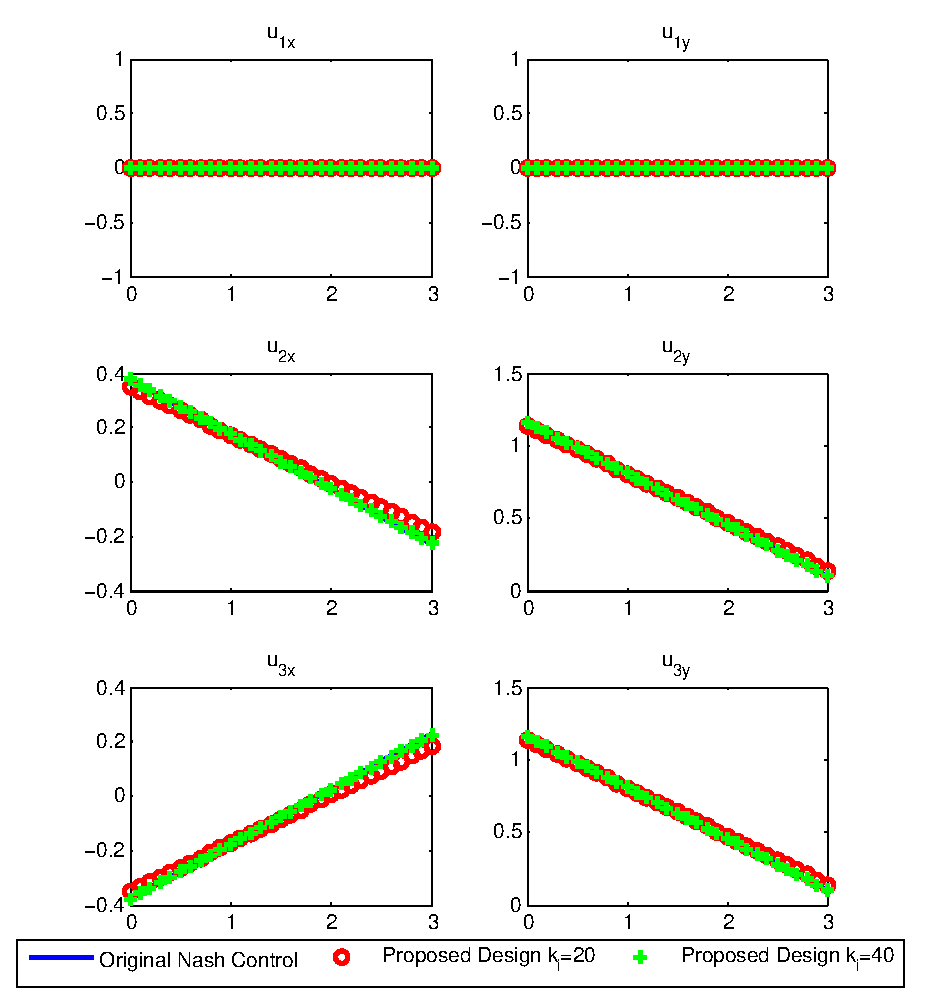
\includegraphics[scale=0.58]{Original_Distributed_control.eps}
      \caption{Nash and proposed designed strategies}\label{Original_Distributed_control}
\end{figure}
The motion trajectories under various control inputs are shown in Figure \ref{TrajectoryUndirected}.
\begin{figure}[h]
      \centering
      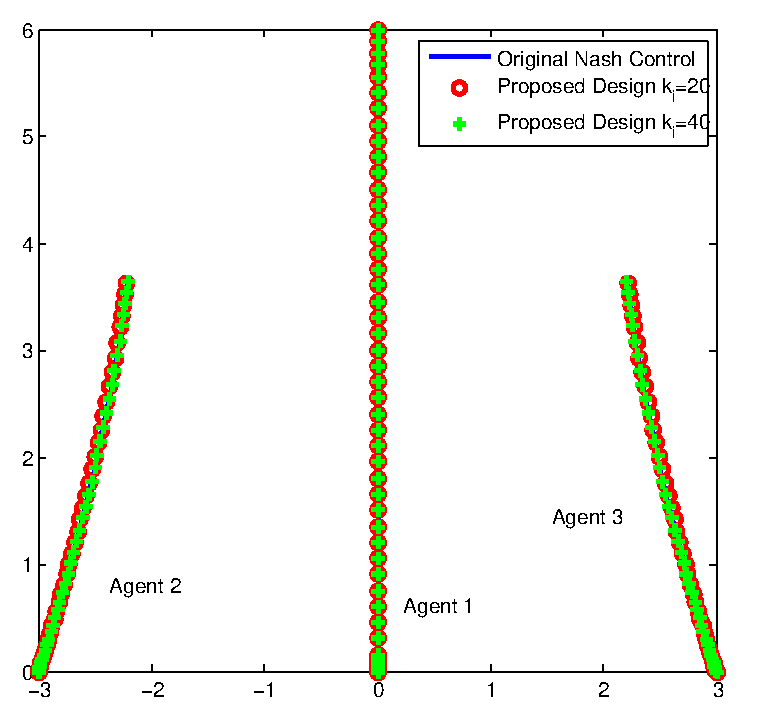
\includegraphics[scale=0.5]{TrajectoryUndirected.eps}
      \caption{Motion trajectories under different control strategies}\label{TrajectoryUndirected}
\end{figure}
Graphically, there does not exist much difference between the trajectories under the original Nash strategies and the ones under designed strategies. Quantitatively, we are able to calculate the total terminal formation error with respect to the desired displaced among the agents, which is
\begin{equation}
\eta=\sum^3_{i=1}\|s_1(t_f)-s_i(t_f)-{\mu_{1i}}\|,
\end{equation}
where $s_i(t_f)$ is agent $i$'s terminal position vector under certain control strategies. Therefore, the total terminal formation errors based on different values of $r_1=r_2=r_3=r$ and $k_1=k_2=k_3=k$ can be summarized into Table \ref{Comparison}.
\begin{table}[h]\normalsize
\centering
\begin{tabular}{|l|c|c|c|}
  \hline
  % after \\: \hline or \cline{col1-col2} \cline{col3-col4} ...
         & Nash & $k=20$ & $k=40$ \\
         \hline
         $\eta\;\;(r=0.2)$ & 0.2162 & 0.2177 & 0.2162 \\
         \hline
  $\eta\;\;(r=1)$ &  0.8164 &  0.8513 & 0.8179 \\
  \hline
  $\eta\;\;(r=5)$ &  2.6541 & 2.6920 & 2.6560 \\
  \hline
\end{tabular}
\caption{Total terminal formation errors in Scenario 1}\label{Comparison}
\end{table}
From the table, it is clear to see that the total terminal formation error decreases as $k_i$ increase because as mentioned, larger $k_i$ will result in more accurate terminal state estimates and more accurate control inputs (with respect to the Nash strategies). It is also clear to see that the total terminal formation error increases as $r$ increases. This is because that if agents put higher penalties on the control effort or energy (i.e., the quadratic term of the control input in (\ref{JiFormation})), they will try to reduce more on control energy instead of the terminal formation errors in order to minimize their performance indices in (\ref{JiFormation}) during the time period of the formation control. Based on more simulation data, the relationship among $\eta$, $k$, and $r$ can be depicted in Figure \ref{Relationship}.
\begin{figure}[h]
      \centering
      \includegraphics[scale=0.5]{PlotT.eps}
      \caption{Relationship among $\eta$, $r$, and $k$}\label{Relationship}
\end{figure}
As we can see in the figure, when $r$ is small, the variance of the total terminal formation error $\eta$ among different $k$ is small, and when $r$ is large, the variance of the total terminal formation error $\eta$ among different $k$ becomes large. Another application of Figure \ref{Relationship} is to determine the lowest update gain $k$ needs to achieve a desired terminal formation error. For instance, if we want to determine a update gain that can achieve a maximum terminal formation error of 2 given $r=2$, then we can find that a value of $k$ less than $6$ is good choice from the figure. Therefore, this figure provides a intuitive way of choosing a proper update gain, especially to avoid choosing a high gain which is undesired in many real life applications.

\textbf{Scenario 2}: We now consider the scenario where there are three agents with undirected communication topology as shown in Figure \ref{Formation3undirected}.
\begin{figure}[h]
      \centering
      \includegraphics[scale=0.8]{Formation3undirected.eps}
      \caption{Three agents with undirected graph}\label{Formation3undirected}
\end{figure}
With this communication topology, both Nash and Pareto strategies can be derived. The initial states of the agents and the performance index parameters are the same as the ones in Scenario 1. For both Nash strategy design and Pareto strategy design, the gain $k_i$ in the terminal state estimation equation (\ref{update}) and (\ref{updatehphv}) are set equal to $40$ for all $i=1,2,3$. For the Pareto strategies, the convex parameters in (\ref{convexcombination}) are set to be $\alpha_1=\alpha_2=\alpha_3=1/3$. The Laplacian matrix for the noncooperative in (\ref{laplacian}) and the one for the cooperative case in (\ref{laplacianFormation}) are
\[\mathcal{L}=\begin{bmatrix}
2&-1&-1\\
-1&1&0\\
-1&0&1
\end{bmatrix}\quad\mbox{and}\quad \mathcal{L}=\begin{bmatrix}
\frac{4}{3}&-\frac{2}{3}&-\frac{2}{3}\\
-\frac{2}{3}&\frac{2}{3}&0\\
-\frac{2}{3}&0&\frac{2}{3}
\end{bmatrix},\]
respectively. The resulting motion trajectories under both Nash and Pareto strategies are shown in Figure \ref{NashPareto}.
\begin{figure}[h!]
      \centering
      \includegraphics[scale=0.5]{NashPareto.eps}
      \caption{Motion trajectories under Nash and Pareto strategies}
      \label{NashPareto}
\end{figure}
The total terminal formation errors under different choices of the convex parameters are summarized in Table \ref{Scenario2Table}.
\begin{table}[h]\normalsize
\centering
\begin{tabular}{|c|c|}
  \hline
  % after \\: \hline or \cline{col1-col2} \cline{col3-col4} ...
       & $\eta$  \\
       \hline
  Nash & 0.4856  \\
  \hline
  Pareto ($\alpha_1=\alpha_2=\alpha_3=1/3$)&0.3033\\
  \hline
  Pareto ($\alpha_1=1/6,\alpha_2=2/3,\alpha_3=1/6$)&0.3128\\
  \hline
  Pareto ($\alpha_1=2/3,\alpha_2=1/6,\alpha_3=1/6$)&0.1791\\
  \hline
  Pareto ($\alpha_1=0.9,\alpha_2=0.05,\alpha_3=0.05$)&0.0602\\
  \hline
\end{tabular}
\caption{Total terminal formation errors in Scenario 2}\label{Scenario2Table}
\end{table}
As we can clearly see in the table, the agents can actually achieve lower formation error using Pareto strategies than using Nash strategies. This is because the agents are assumed to cooperate with each other in the Pareto optimality. Also note that as we place more weight on agent $1$'s performance index, the total formation error can be reduced. This is because it is much easier to move agent 1 alone to form the desired formation {instead} of moving all the three agents together.
%%%%%%%%%%%%%%%%%%%%%%%%%%%%%%%%%%%%%%%%%%%%%%%%%%%%%%%%%%%%%%%%%%%%%%%%%%%%%%%%

\section{Conclusion}\label{conclusion}
{This paper considers the design of open-loop Nash and Pareto strategies for multi-agent formation control problems. The proposed approach utilizes the distributed estimation of the terminal state variables among the agents through network-based information exchange. The convergence rate of the terminal state estimation algorithm is determined by a scalar gain and can be made sufficiently fast to get a better approximation of the real Nash and Pareto strategies. An illustrative example is solved with two scenarios and various comparisons have been made.}

%\addtolength{\textheight}{-12cm}% This command serves to balance the column lengths
                                  % on the last page of the document manually. It shortens
                                  % the textheight of the last page by a suitable amount.
                                  % This command does not take effect until the next page
                                  % so it should come on the page before the last. Make
                                  % sure that you do not shorten the textheight too much.
%
%Appendixes should appear before the acknowledgment.

\appendix

First of all, we present the following lemmas:
\begin{Lem}\label{LemmaEigen}
All eigenvalues of $S_{ii}$ in (\ref{dSkd}) have nonnegative real parts.
\end{Lem}
\begin{proof}
Substituting (\ref{Sk}) into (\ref{dSkd}) yields
\begin{align*}
S_{ii}
&=(e_i^T\otimes I_r) \int^{t_f}_0
B'_iR_i^{-1}(B'_i)^T \mbox{d}t
D_j^T\tilde{F}_j(e_i\otimes I_k).
\end{align*}
Due to the definition of $D_j$ in (\ref{Di}) and $\tilde{B}_j=(d_j\otimes
I_r)B'_j$, the above equation becomes
\begin{align*}
S_{jj}=\underbrace{\int^{t_f}_0 B'_j(t)R_j^{-1}(t)(B'_j)^T(t)\mbox{d}t}_a
\underbrace{ (d_j^T\otimes I_r)\tilde{F}_j(d_j\otimes I_k)}_b.
\end{align*}
Since both term $a$ and term $b$ are positive semi-definite, all the
eigenvalues of matrix $S_{jj}$ have nonnegative real parts.
\end{proof}

\begin{Lem}\label{norminequality}
If $(-M)$ is Hurwitz for matrix $M$ defined in (\ref{M}), supposing that matrix $P$ is the unique positive definite solution to the Lyapunov equation
\begin{equation}
-M^TP-PM=-I,\label{lyapunov}
\end{equation}
then for linear system
\begin{equation}
\dot{\theta}=-gM\theta\label{theta}\\
\end{equation}
with the initial state $\theta(0)$, the inequalities
\begin{subequations}\label{thetainequalitytotal}
\begin{align}
&\int^{t_f}_0\|\theta\|_2^2\mbox{d}t\leq \frac{2\gamma_{\max}V(0)}{g\gamma_{\min}} (1-e^{-g\gamma_{\min}t_f}),\label{thetainequality2}\\
&\int^{t_f}_0\|\theta\|_2\mbox{d}t\leq  \frac{2\sqrt{2\gamma_{\max}V(0)}}{g\gamma_{\min}} (1-e^{-g\gamma_{\min}t_f/2})\label{thetainequality}.
\end{align}
\end{subequations}
hold, where $\|\cdot\|_2$ stand for Euclidean norm, $V(0)=1/2\theta^T(0)P\theta(0)$, $\gamma_{\min}=1/\lambda_{\max}(P)$, $\lambda_{\max}(P)$ is the largest eigenvalue of matrix $P$, $\gamma_{\max}=1/\lambda_{\min}(P)$, and $\lambda_{\min}(P)$ is the smallest eigenvalue of matrix $P$.
\end{Lem}
\begin{proof}
If matrix $(-M)$ is Hurwitz, we consider the quadratic Lyapunov function $V=1/2\theta^TP\theta$ for system (\ref{theta}), where matrix $P$ is the solution to the Lyapunov equation (\ref{lyapunov}). The derivative of the Lyapunov function along the trajectory of system (\ref{theta}) is
\[\dot{V}=\frac{1}{2}\theta^T(-gM^TP-gPM)\theta= -\frac{g}{2}\|\theta\|^2_2\leq -\frac{g}{2\lambda_{\max}(P)}\theta^TP\theta= -g\gamma_{\min} V\]
where the last inequality is due to the property $\theta^TP\theta\leq \lambda_{\max}(P)\|\theta\|_2^2$. The above differential inequality yields
\begin{align*}
&\frac{1}{2}\lambda_{\min}(P)\|\theta\|_2^2\leq \frac{1}{2}\theta^TP\theta=V(t)\leq e^{ -g\gamma_{\min} t}V(0)\quad
\Longrightarrow\quad \|\theta\|^2_2\leq 2\gamma_{\max}e^{ -g\gamma_{\min} t}V(0).
\end{align*}
Therefore, integrating the above inequality from $0$ to $t_f$ yields (\ref{thetainequality2}) and the square root of the above inequality from $0$ to $t_f$ yields (\ref{thetainequality}).
\end{proof}

\begin{Lem}
Under strategy , $\Delta x_i$ can be expressed as
\end{Lem}
\begin{proof}
Since $\Delta x_i(t_f)=x_i(t_f)-x_i^*(t_f)$, we need to find expressions for both $x_i(t_f)$ and $x_i^*(t_f)$. For $x_i(t_f)$, we solve differential equation (\ref{stacked}) as
\[\dot{x}_{f}(\tau)=G\left\{[I_N\otimes\Phi(t_f,0)]x(0)-(I+DL)x_f(\tau)+D\mu\right\},\]
\begin{equation}
z^f(t)=M^{-1}z(0)+\theta(t).\label{zfsolution}
\end{equation}
where $\theta(t)$ is defined in (\ref{theta}) with the initial state $\theta(0)=z^f(0)-M^{-1}z(0)$. The system dynamics
(\ref{dynamiczi}) when every agent chooses strategy
(\ref{OpenLoopNashAlgorithm2}) becomes
\begin{equation}
\dot{z}= -\sum^N_{j=1}\tilde{B}_jR^{-1}_j\tilde{B}_j^T
D_i^T\tilde{F}_jD_jz^f\triangleq -Wz^f\label{zdotzf}
\end{equation}
where $W$ is defined in (\ref{Wmax}). Substituting (\ref{zfsolution}) into
(\ref{zdotzf}) yields
\begin{equation}
\dot{z}=-WM^{-1}z(0)-W\theta.  \label{zdotzfz0}
\end{equation}
Since
\[\int^{t_f}_0W\mbox{d}t=\sum^N_{j=1}S_jF_j\]
where matrices $F_j$ and $S_j$ are defined in (\ref{Fi}) and (\ref{Sk}),
integrating equation (\ref{zdotzfz0}) from $0$ to $t_f$ yields
\begin{equation}
z(t_f)=\left(I-\sum^N_{j=1}S_jF_jM^{-1}\right)z(0)
-\int^{t_f}_0W\theta\mbox{d}t. \label{xtf}
\end{equation}
Recalling the definition of matrix $M$ in (\ref{M}), we have
\[\left(I+\sum^N_{j=1}S_jF_j\right)M^{-1} =I\quad\Longrightarrow\quad
M^{-1}=I-\sum^N_{j=1}S_jF_jM^{-1}.\]
Hence, equation (\ref{xtf}) becomes
\begin{equation}
z(t_f)=M^{-1}z(0) -\int^{t_f}_0W\theta\mbox{d}t. \label{xtf1}
\end{equation}
%and
%\[x_j(t_f)=(d_i^T\otimes I_n)(I+S)^{-1}x(0)-(d_i^T\otimes
%I_n)\int^{t_f}_0We^{-K(I+S)t}\mbox{d}t[\alpha(0)-(I+S)^{-1}x(0)]\]
Second, substituting $u^*_i$ in (\ref{uibest}) into (\ref{zidot}) yields
\[\dot{z}^*_i=-(d_i^T\otimes
I_r)\tilde{B}_iR_i^{-1}\tilde{B}_i^TD_i^T\tilde{F}_i \left[
D_iz(t_f)-(d_i\otimes I_r)\Delta z_i(t_f)\right]\]
Integrating the above equation from $0$ to $t_f$ yields
\begin{align*}
z_i^*(t_f)=&z_i(0)-(d_i^T\otimes I_r)S_iD_i^T\tilde{F}_i\left[
D_iz_i(t_f)-(d_i\otimes I_r)\Delta z_i(t_f)\right]\\
=&z_i(0)+S_{ii}\Delta z_i(t_f)-(d_i^T\otimes I_r)S_iF_iz(t_f)
\end{align*}
where $S_{ii}$ is as defined in (\ref{dSkd}). Therefore, substituting the
above equation into the expression of $\Delta z_i(t_f)$ yields
\begin{align*}
\Delta z_i(t_f)=&z_i(t_f)-z_i^*(t_f)=z_i(t_f)-z_i(0)-S_{ii}\Delta
z_i(t_f)+(d_i^T\otimes I_r)S_iF_iz(t_f)
\end{align*}
After some manipulations, we arrive at
\begin{align*}
(I+S_{ii})\Delta z_i(t_f)=&(d_i^T\otimes I_n)[Mz(t_f)-z(0)]
\end{align*}
As we showed in Lemma \ref{LemmaEigen}, all the eigenvalues of $S_{ii}$ in the
right hand side of the above equation have nonnegative real parts and hence
matrix $(I+S_{ii})$ is invertible. Therefore,
\begin{equation}
\Delta z_i(t_f)=(I+S_{ii})^{-1}(d_i^T\otimes I_r)\left[Mz(t_f)-z(0)\right]
\label{Deltazitf}
\end{equation}
Therefore, substituting (\ref{xtf1}) into (\ref{Deltazitf}) yields the value
of $\Delta z_i(t_f)$ as follows:

\end{proof}


\begin{Lem}
$\Delta u_i$
\end{Lem}
\begin{proof}
The value of $\Delta u_i$ obtained as follows:
\begin{align}
\Delta u_i=u_i-u_i^*=&-R^{-1}_i\tilde{B}_i^TD_i^T\tilde{F}_iD_iz^f
+R^{-1}_i\tilde{B}_i^TD_i^T\tilde{F}_iD_iz^*(t_f)\notag\\
=&-R^{-1}_i\tilde{B}_i^TD_i^T\tilde{F}_iD_iz^f
+R^{-1}_i\tilde{B}_i^TD_i^T\tilde{F}_iD_iz(t_f)
-R_i^{-1}\tilde{B}_iD_i^T\tilde{F}_i(d_i\otimes I_r)\Delta z_i(t_f)\notag\\
=&-R^{-1}_i\tilde{B}_i^TD_i^T\tilde{F}_iD_i[z^f-z(t_f)]
-R_i^{-1}\tilde{B}_iD_i^T\tilde{F}_i(d_i\otimes I_r)\Delta
z_i(t_f)\label{Deltaui},
\end{align}
Recalling (\ref{zf}) and (\ref{xtf1}), the value of $[z^f-z(t_f)]$ in the
above equation can be obtained as
\begin{align}
z^f-z(t_f)=&\theta+\int^{t_f}_0W\theta\mbox{d}t\label{zfztf}
\end{align}
Substituting (\ref{Deltazitf1}) and (\ref{zfztf}) into (\ref{Deltaui}) yields
\[\triangleq  -R^{-1}_i\tilde{B}_i^TD_i^T\tilde{F}_iD_iv_i\]
where
$v_i=\theta+ M_i\int^{t_f}_0W\theta\mbox{d}t$ and matrix $M_i$ is
defined in (\ref{MiN}). 
\end{proof}

%\section*{ACKNOWLEDGMENT}


\bibliographystyle{IEEEtran}
\bibliography{Mybib}




\end{document}
